\chapter{Эквивалентные условия правильности семейств}\label{sec:equivalence}

\epigraph{Математика — это искусство называть разные вещи одним и тем же именем.}{Жюль Анри Пуанкаре}

\section{Одностоковые ориентации булевых кубов}
\label{sec:uso}
    В данном разделе мы приведем характеризацию правильных семейств булевых функций в геометрических терминах, а именно, в терминах ориентации, индуцируемой булевым правильным семейством на графе булева куба.

\subsection{Определение одностоковых ориентаций}
    Для начала дадим необходимые предварительные определения.

    \begin{definition}
        Графом булева куба $G(\EE_2^n)$ размерности $n$ будем называть граф на $2^n$ вершинах с метками $(\alpha_1, \ldots, \alpha_n)$, $\alpha_i \in \{0, 1\}$, где ребра проведены между вершинами, расстояние Хэмминга (см. раздел~\ref{sec:discretefunctions}) между которыми равно 1.
    \end{definition}

    \begin{definition}
        Подкубом булева куба размерности $(n - m)$ будем называть подграф графа $G(\EE_2^n)$, порожденный вершинами с фиксированными значениями некоторых координат $i_1, \ldots, i_m \in \{1, \ldots, n\}$.
        В частности, подкубами размерности 1 являются ребра графа булева куба $G(\EE_2^n)$, 
        подкубами размерности 2~--- всевозможные двумерные грани куба $G(\EE_2^n)$ и так далее.
    \end{definition}

    \begin{definition}
        Стоком в ориентированном графе будем называть вершину, в которую входят ребра и из которой не исходят ребра.
    \end{definition}

    Следующее определение было введено в работе~\cite{szabo2001} в контексте изучения задач оптимизации.
    \begin{definition}
        Реберной ориентацией с единственным стоком на графе булева куба $G(\EE_2^n)$ называется ориентация всех ребер графа $G(\EE_2^n)$ с таким свойством, что в каждом подкубе размерностей $m = 1, 2, \ldots, n$ существует ровно 1 сток. 
    \end{definition}

    Для краткости будем в дальнейшем называть такие ориентации одностоковыми (или $\uso$-ориентациями, \textbf{U}nique \textbf{S}ink \textbf{O}rientation).
    Примеры одностоковых ориентаций кубов приведены на рисунках~\cref{fig:cube2, fig:cube3}.
    \begin{figure}[ht] % Рисунок
        \centerfloat{
            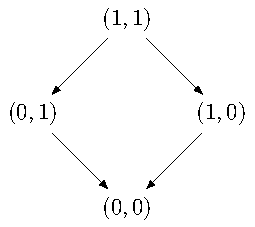
\includegraphics[scale = 0.8]{fig0}
            \caption{Одностоковая ориентация двумерного куба $G(\EE_2^2)$}\label{fig:cube2}
        }
    \end{figure}


    \begin{figure}[ht] % Рисунок
        \centerfloat{
            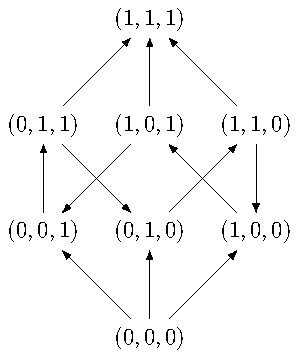
\includegraphics[scale = 0.8]{fig1}
            \caption{Одностоковая ориентация трехмерного куба $G(\EE_2^3)$}\label{fig:cube3}
        }
    \end{figure}

    \begin{definition}
        Пусть задано семейство булевых функций $\ff_n$ размера $n$, в котором функция $f_i$ не зависит существенно от $x_i$, $1 \le i \le n$.
        Тогда семейство $\ff_n$ индуцирует на $G(\EE_2^n)$ ориентацию ребер следующим образом.
        Пусть $(\uu, \vv)$~--- смежные вершины в $G(\EE_2^n)$, различающиеся в $i$-м бите. 
        Рассмотрим значение $i$-й функции семейства $\ff_n$ на этих двух наборах. 
        Поскольку $f_i$ не зависит существенно от одноименной переменной $x_i$, то $f_i(\uu) = f_i(\vv)$. 
        Если $f_i(\uu) = u_i$, то ребро ориентируется от $\vv$ к $\uu$, в противном случае ($f_i(\uu) = v_i$) ребро ориентируется от $\uu$ к $\vv$.
    \end{definition}

    \begin{definition}
        Полученный выше ориентированный граф (граф $G(\EE_2^n)$ с дополнительно индуцированной семейством $\ff_n$ ориентацией ребер) называется асинхронным графом семейства (или асинхронной булевой сетью) $\ff_n$ и обозначается $\Gamma_{\ff_n}$.
    \end{definition}

    \begin{remark}
    \label{rem:fixpt_uso}
        Нетрудно заметить, что вершина $\yy$ является стоком в графе $\Gamma_{\ff_n}$ тогда и только тогда, когда $\yy$~---~неподвижная точка отображения $\ff_n \colon \EE_2^n \to \EE_2^n$.
        Действительно, $\ff(\yy) = \yy$ тогда и только тогда, когда $f_i(\yy) = y_i$ для каждого $i = 1, \ldots, n$, что, в свою очередь, равносильно тому, что $\yy$ является стоком в описанном графе.
    \end{remark}

    \begin{remark}
        Соответствие между семействами $\ff = (f_1, \ldots, f_n)$ булевых функций (где $f_i$ не зависит существенно от $x_i$) и асинхронными графами семейств $\Gamma_{\ff}$ является взаимно-однозначным.
        \begin{enumerate}
            \item По семейству однозначно задается (указанным выше способом) ориентация на графе булева куба $G(\EE_2^n)$;
            \item По ориентированному графу булева куба $\Gamma_{\ff}$ можно восстановить значение всех функций семейства на любом $\xx \in \EE_2^n$: рассмотрим вершину с меткой $\xx$ и все смежные с ней ребра.
            Если $i$-е ребро (ребро, ведущее из вершины $\xx$ в вершину, отличную от $\xx$ в $i$-й координате) выходит из $\xx$, то $f_i(\xx) = \overline{x_i}$, иначе $f_i(\xx) = x_i$.
            В полученном семействе $f_i$ не зависит существенно от $x_i$, поскольку ни одно ребро не ориентировано в две стороны.
        \end{enumerate}
    \end{remark}

\subsection{Неподвижные точки правильных семейств}
    
    \begin{lemma}[{\cite[лемма~2]{pdm20}}]
    \label{lemma:fixpt}
        У правильного семейства булевых функций всегда существует единственная неподвижная точка.
    \end{lemma}

    \begin{proof}
        Будем вести доказательство индукцией по размеру правильного семейства. 
        Булевы семейства размера $n = 1$~--- это константы $a \in \EE_2^n$, для них утверждение тривиально выполнено.

        Рассмотрим семейство $\ff_n$ размера $n$.
        Рассмотрим его проекции $\proj^0_n(\ff_n)$ и $\proj^1_n(\ff_n)$, которые также являются правильными семействами (предложение~\ref{thm:proj}).
        По предположению индукции для указанных проекций в каждом подкубе существует единственная неподвижная точка:
        \begin{gather*}
            \alpha = (\alpha_1, \ldots \alpha_{n-1}, 0), \\
            \beta = (\beta_1, \ldots \beta_{n-1}, 1),
        \end{gather*}
        то есть, выполнены равенства:
        \begin{gather*}
            f_1(\alpha) = \alpha_1, \ldots, f_{n-1}(\alpha) = \alpha_{n-1}, \\
            f_1(\beta) = \beta_1, \ldots, f_{n-1}(\beta) = \beta_{n-1}.
        \end{gather*}
        Рассмотрим значения $f_n(\alpha)$ и $f_n(\beta)$. 
        Так как семейство $\ff_n = (f_1, \ldots, f_n)$~--- правильное, то найдется индекс $j \in \{1, \ldots n\}$, такой что $\alpha_j \ne \beta_j$, $f_j(\alpha) = f_j(\beta)$. 
        Из приведенных выше рассуждений видно, что единственный случай, когда данное условие может быть выполнено~---~ случай $j = n$. 
        В таком случае, если $f_j(\alpha) = 0$, то единственной неподвижной точкой является $\alpha$, иначе такой точкой является точка $\beta$.
    \end{proof}

    Следующая теорема устанавливает взаимно-однозначное соответствие между правильными семействами булевых функций размера $n$ и $\uso$-ориентациями булевых кубов размерности $n$.
    \begin{theorem}[{\cite[теорема~2]{pdm20}}]
        Граф семейства $\Gamma_{\ff}$ является одностоковой ориентацией булева куба $\EE_n$ тогда и только тогда, когда $\ff$~--- правильное семейство.
    \end{theorem}

    \begin{proof}
        Как было отмечено выше, стоки в графе $\Gamma_{\ff}$ соответствуют неподвижным точкам ограничения отображения $\ff$ на соответствующий подкуб куба $\EE_n$. 

        Пусть $\ff_n$~---~правильное булево семейство. 
        Тогда по теореме~\ref{thm:proj} любая проекция семейства $\ff$ на любой подкуб $\EE_n$ также является правильным семейством. 
        По лемме~\ref{lemma:fixpt} такое ограничение имеет единственную неподвижную точку в данном подкубе, т.е. данный подкуб имеет единственный сток. 
        Следовательно, граф $\Gamma_{\ff}$ для правильного семейства $\ff$ является одностоковой ориентацией. 

        Докажем утверждение в обратную сторону. 
        Пусть $\Gamma_{\ff}$~--- одностоковая ориентация. 
        Покажем по индукции, что в этом случае $F$ является правильным семейством. 

        \textbf{База индукции:} при $n = 1$ нетрудно убедиться, что существует ровно две одностоковые ориентации на двух вершинах, соответствующие константным (а значит, правильным) семействам размера 1:
        \begin{equation*}
            \ff^0 = 
            \begin{bmatrix}
                0
            \end{bmatrix}, \quad
            \ff^1 = 
            \begin{bmatrix}
                1
            \end{bmatrix}.
        \end{equation*}

        \textbf{Индукционный переход:} пусть $\alpha \ne \beta$, где $\alpha, \beta \in \EE_2^n$.
        По определению правильного семейства мы должны показать, что тогда существует индекс $i$, такой что $\alpha_i \ne \beta_i$, но $f_i(\alpha) = f_i(\beta)$.
        Если найдется индекс $k$, такой что $\alpha_k = \beta_k$, то задача может быть сведена к задаче меньшей размерности: рассмотрим проекцию на подкуб $x_k = \alpha_k$ и используем индукционное предположение.
        
        Следовательно, можем считать, что $\alpha_k \ne \beta_k$, $1 \le k \le n$. 
        Дополнительно мы можем считать, что $\alpha$~--- сток, то есть $f_k(\alpha) = \alpha_k$, $1 \le k \le n$. 
        Если это не так, то мы можем перейти к новому семейству $g_k(\xx) = f_k(\xx) \oplus 1$, таким образом изменив направление всех ребер между подкубами ${x_k = 0}$ и $x_k = 1$. 
        Данная смена направлений ребер не разрушает свойство ориентации быть одностоковой. 
        В силу теоремы~\ref{thm:outer_shift} указанное преобразование не нарушает правильность семейства.
        Таким образом, можно без ограничения общности считать, что вершина $\alpha$ является стоком.

        Но в таком случае если $f_k(\alpha) \ne f_k(\beta)$, $1 \le k \le n$, то мы имеем $f_k(\beta) = \beta_k$, $1 \le k \le n$, то есть вершина $\beta$ также является стоком, что противоречит одностоковости. 
        Следовательно, должен найтись какой-либо индекс $k$, для которого $f_k(\alpha) = f_k(\beta)$, что и требовалось доказать.
    \end{proof}

    Таким образом, учитывая то, что стокам в $\uso$-ориентациях соответствуют неподвижные точки семейства (см. замечание~\ref{rem:fixpt_uso}), был получен следующий критерий правильности семейства: семейство булевых функций $\ff_n$ правильно тогда и только тогда, когда каждое подсемейство семейства $\ff_n$ (в том числе и само исходное семейство) имеет единственную неподвижную точку (см. также раздел~\ref{sec:hupfnet}). 
    В работе~\cite{fpm23} (см. теорему~2) было показано, что данный критерий нельзя напрямую распространить с булева случая на случай $k$-значной логики, где $k \ge 3$.
    Более точно, было показано, что если семейство $\ff_n$ в $k$-значной логике является правильным, то у него и всех его проекций существует единственная неподвижная точка, однако обратное утверждение неверно: так, например, для семейства
    \begin{equation*}
        \begin{bmatrix}
            f_1(x_1, x_2) \\
            f_2(x_1, x_2)
        \end{bmatrix} = 
        \begin{bmatrix}
            2x_2 \\
            x_1
        \end{bmatrix}
    \end{equation*}
    выполняется свойство единственности неподвижной точки для всех возможных подсемейств, однако семейство не является правильным (см.~\cite{galatenko21criterion}).
    Обобщение критерия может быть сформулировано в терминах перекодировок исходного семейства (см. раздел~\ref{sec:reencoding} и утверждение~\ref{thm:reencoding_properness}).

\subsection{Оценки на число правильных булевых семейств}

    Обозначим через $T_k(n)$ количество правильных семейств в $k$-значной логике размера $n$ (если $k = 2$, то индекс $k$ будем опускать).

    \begin{corollary}[{\cite[лемма~6.10]{USOphd}}]
    \label{uso:lowerbound}
        Выполнение следующее неравенство 
        \[
            T(n) \ge 4 \left( T(n-1) \right)^2.
        \]
    \end{corollary}

    Отметим, что оценка вида $T(n) \ge 2 \left( T(n-1) \right)^2$, или, более общо, 
    \[
        T_k(n) \ge k \cdot \left( T_k(n-1) \right)^k
    \] 
    для случая $k$-значной логики может быть получена за счет явных конструкций построения новых правильных семейств из старых (см., например,~\cite[теорема~2]{galatenko20algo}).

    % TODO: неужели не получается обобщить на k-значную логику?

    % Результат из следствия~\ref{uso:lowerbound} можно усилить на случай $k$-значной логики.
    % Доказательство является адаптацией рассуждений из работы~\cite{USOphd} на язык правильных семейств.
    % \begin{corollary}
    % \label{uso:klowerbound}
    %     Обозначим за $T_k(n)$ количество правильных семейств $k$-значной логики размера $n$. 
    %     Тогда $T_k(n+1) \ge k^2 (T_k(n))^k$. 
    % \end{corollary}

    % \begin{proof}
    %     Рассмотрим процедуру построения семейства размера $n+1$ из семейств размера $n$.
    %     Для начала построим $k$ <<рекурсивных>> ориентаций: пусть $\ff^i_{n}$, $0 \le i \le k-1$~--- $k$ правильных семейств размера $n$.

    %     Зададим функцию $f_{n+1}(x_1, \ldots, x_{n+1}) \equiv a$, где $a \in \EE_k$~--- произвольный элемент, и зададим семейство размера $n+1$ как:
    %     \[
    %         \ff_{n+1}(x_1, \ldots, x_{n+1}) = 
    %         \begin{bmatrix}
    %             \bigvee_{0 \le j \le k-1} \II_{x_{n+1}}(j) \wedge \ff^i_{n}(x_1, \ldots, x_n) \\
    %             a
    %         \end{bmatrix}.
    %     \]
    %     Заметим, что проекции $\ff_{n+1}$ вида $x_{n+1} \gets b$, $0 \le b \le k-1$ имеют вид:
    %     \[
    %         \proj^{b}_{n+1} \left( \ff_{n+1} \right) = \ff^b_n(x_1, \ldots, x_n).
    %     \]
    %     Указанным образом можно получить $k$ различных правильных семейств для каждой фиксации набора правильных семейств $\ff^j_n$, $0 \le j \le n-1$, а значит, общее число получаемых таким образом семейств размера $n+1$ равно 
    %     \[
    %         k \cdot (T_k(n))^k.
    %     \] 

    %     Теперь рассмотрим построение не-рекурсивных семейств.
    %     Возьмем произвольные точки $v_1, \ldots, v_k \in \EE_k^n$ и произвольное правильное семейства $\ff^0$ размера $n$.
    %     Рассмотрим множества правильных семейств, которые в заданной точке $\xx$ принимают заданное значение $\vv$:
    %     \[
    %         V(\xx, \vv) = \{\ff_n \mid \ff_n(\xx) = \vv \}.
    %     \]
    %     Заметим, что множества $V(\xx, \vv)$ не пересекаются и равномощны для разных значений $\vv$, поскольку множество $V(\xx, \ww)$, $\ww \ne \vv$ можно получить сдвигом всех функций $V(\xx, \vv)$ на вектор значений $\ww - \vv$, а значит:
    %     \[
    %         V(\xx, \vv) = \frac{T_k(n)}{k^n}.
    %     \]
    %     По выбранному семейству $\ff^0$ выберем семейства $\ff^1, \ldots, \ff^k$ таким образом, что $\ff^j(\vv_j) = \ff^0(\vv_j)$; другими словами:
    %     \[
    %         \ff^j \in V(\vv_j, \ff^0(\vv_j)).
    %     \]
    %     Построим семейство размера $n+1$ следующим образом:
    %     \[
    %         \ff_{n+1}(x_1, \ldots, x_{n+1}) = 
    %         \begin{bmatrix}
    %             \bigvee_{0 \le j \le k-1} \II_{x_{n+1}}(j) \wedge \ff^i(x_1, \ldots, x_n) \\
    %             f_{n+1}(x_1, \ldots, x_n)
    %         \end{bmatrix}.
    %     \]
    %     Поскольку проекции семейства $\ff_{n+1}$ различны при различных $\ff^0, \ldots, \ff^k$, то при каждой фиксации последних мы будем получать некоторое отличное от предыдущих построенных семейство размера $n+1$.
    %     Зададим функцию $f_{n+1}$ следующим образом:
    %     \begin{itemize}
    %         \item если $\xx_0 \not \in \{\vv_1, \ldots, \vv_k\}$, то положить $f_{n+1}(\xx_0) = a$,
    %         \item положить $f_{n+1}(\vv_j) = a_j$.
    %     \end{itemize}
    %     Полученное таким образом семейство будет правильным при любом выборе $a$ и $a_j$:
    %     \begin{itemize}
    %         \item если два набора $\xx$ и $\yy$ отличаются в $n+1$-й координате 
    %     \end{itemize}



    % \end{proof}

    

    \begin{proposition}[{\cite[теорема~1]{numberUSO}}]
    \label{thm:num_of_proper}
        Cуществуют константы $B \ge A > 0$, такие что для $n \ge 2$ выполняются неравенства:
        \[ 
            n^{A \cdot 2^n} \le T(n) \le n^{B \cdot 2^n}.
        \]
    \end{proposition}

    В частности, из этого результата следует, что доля булевых правильных семейств даже среди булевых семейств, для которых $f_i$ не зависит существенно от $x_i$ (необходимое условие правильности, см. замечание~\ref{rem:essential_general}), является экспоненциально малой.

    Также, используя полученную выше оценку, можно показать, что число треугольных семейств среди правильных есть $o(1)$ при стремлении размера семейства $n \to \infty$, а именно, что доля треугольных семейств среди правильных убывает со скоростью ${n^{-D \cdot 2^n}}$, где $D > 0$ (т.е. экспоненциально мала).

    \begin{theorem}[{\cite[теорема~6]{dm21}}]
    \label{thm:triangle}
        Обозначим через $\Delta(n)$ количество булевых треугольных семейств размера $n$.
        Тогда:
        \[
            \frac{\Delta(n)}{T(n)} = o \left(\frac{1}{n^{D \cdot 2^n}} \right)
            \text{ при } n \to \infty
        \]
        для некоторого $D > 0$.
    \end{theorem}

    Докажем несколько вспомогательных утверждения (верхнюю и нижнюю оценки на число $\Delta(n)$, а также техническую лемму, необходимую для оценки).

    \begin{lemma}[{\cite[лемма~3]{dm21}}]
    \label{lemma:seriessum}
        Выполнено неравенство:
        \[
            \sum_{k=2}^{\infty} \frac{k}{2^{2^{k-1}}} < 0.705.
        \]
    \end{lemma}

    \begin{proof}
        С помощью компьютерных вычислений можно убедиться, что: 
        \[
            \sum_{k=2}^{10} \frac{k}{2^{2^{k-1}}} < 0.704.
        \]
        Остаток ряда можно оценить следующим образом:
        \[
            \sum_{k=11}^{\infty} \frac{k}{2^{2^{k-1}}} < \sum_{k=11}^{\infty} \frac{1}{2^k} < 0.001,
        \]
        поскольку для каждого члена ряда выполнено неравенство (при $k>4$):
        \[
            \frac{k}{2^{2^{k-1}}} < \frac{1}{2^k} 
            \Leftrightarrow
            k \cdot 2^k < 2^{2^{k-1}}.
        \]
    \end{proof}


    \begin{lemma}[{\cite[лемма~1]{dm21}}]
        \label{lemma:num_triangle}
        Выполнено следующее неравенство:
        \[
            \Delta(n) \le n! \cdot 2^{2^n - 1}.
        \]
    \end{lemma}

    \begin{proof}
        Зафиксируем подстановку $\sigma \in \SSS_n$ и оценим сверху число булевых функций, которые могут стоять на позиции $\sigma(m)$ как $2^{2^{m-1}}$, поскольку функция с номером $\sigma(m)$ зависит существенно не более чем от $m-1$ переменной.
        В таком случае общее число треугольных семейств не превышает:
        \[
            \Delta(n) \le n! \cdot 2^{2^0} \cdot 2^{2^1} \cdot \ldots \cdot 2^{2^{n-1}} = n! \cdot 2^{2^n-1}.
        \]
    \end{proof}

    Заметим, что некоторые семейства при такой оценке могли быть подсчитаны более одного раза. 
    Тем не менее, оценка является достаточно точной, а именно, выполняется следующее утверждение.

    \begin{lemma}[{\cite[лемма~2]{dm21}}]
        \label{lem:lower_bound}
        Выполнено следующее неравенство:
        \[
            \Delta(n) \ge 0.145 \cdot n! \cdot 2^{2^n-1}.
        \]
    \end{lemma}

    \begin{proof}
        За $e(n)$ обозначим число $n$-местных булевых функций, существенно зависящих от всех $n$ переменных.
        Тогда количество треугольных семейств может быть оценено снизу как:
        \[
            \Delta(n) \ge n! \cdot e(0) \cdot e(1) \cdot \ldots \cdot e(n-1),
        \]
        поскольку в данном случае мы подсчитываем число треугольных семейств, в которых после упорядочивания первая функция существенно зависит ровно от $0$ переменных, вторая функция зависит существенно ровно от одной переменной $x_{\sigma(1)}$ и так далее. 
        При этом при различных $\sigma$ мы получаем заведомо различные семейства. 
        Необходимо оценить снизу полученное произведение.

        Можно оценить число $e(n)$ снизу следующим образом:
        \[
            e(n) \ge 2^{2^n} - n \cdot 2^{2^{n-1}}.
        \]
        Данная оценка получается из следующих соображений: из множества всех булевых функций от $n$ переменных $x_1, \ldots, x_n$ вычтем все функции, которые зависят только от $n-1$ выбранной переменной (имеется $n$ способов зафиксировать одну переменную, от которой не будет зависеть функция).

        При этом данная оценка является оценкой снизу, поскольку некоторые функции учитываются более одного раза в вычитаемом (например, функции, не зависящие одновременно от двух переменных).

        Таким образом,
        \begin{multline*}
            \frac{\Delta(n)}{n! \cdot 2^{2^0} \cdot 2^{2^1} \cdot \ldots \cdot 2^{2^{n-1}}} \ge 
            \frac{e(0)}{2^{2^0}} \times \ldots \times \frac{e(n-1)}{2^{2^{n-1}}} \ge \\
            \ge 1 \cdot \left( 1 - \frac{1}{2^{2^0}} \right) \cdot 
            \left( 1 - \frac{2}{2^{2^1}} \right) \times 
            \ldots \times 
            \left( 1 - \frac{n-1}{2^{2^{n-2}}} \right) \ge \\
            \ge \frac{1}{2} \cdot \left( 1 - \left( \frac{2}{2^{2^1}} + \ldots + \frac{n-1}{2^{2^{n-2}}} \right) \right) \ge \\
            \ge \frac{1}{2} \left( 1 - \sum_{k=2}^{\infty} \frac{k}{2^{2^{k-1}}} \right).
        \end{multline*}

        Для завершения доказательства леммы~\ref{lem:lower_bound} остается воспользоваться оценкой сверху для ряда $\sum_{k=2}^{\infty} \frac{k}{2^{2^{k-1}}}$.
        Используя лемму~\ref{lemma:seriessum}, получим:
        \[
            \frac{1}{2} \left( 1 - \sum_{k=2}^{\infty} \frac{k}{2^{2^{k-1}}} \right) \ge \frac{1}{2}(1 - 0.705) = 0.1475,
        \]
        откуда следует утверждение леммы \ref{lem:lower_bound}.
    \end{proof}

    Таким образом, можно утверждать, что при $n \to \infty$ имеется оценка:
    \[
        \Delta(n) = \Theta \left( n! \cdot 2^{2^n-1} \right).
    \]
    Перейдем к доказательству теоремы~\ref{thm:triangle}.

    \begin{proof}
        Используя нижнюю оценку из следствия~\ref{thm:num_of_proper} и формулу Стирлинга (см., например,~\cite[часть~II, параграф~4]{yablonski}), можно оценить долю треугольных семейств среди правильных:

        \begin{multline*}
            \frac{\Delta(n)}{T(n)} \le \frac{n! \cdot 2^{2^n - 1}}{n^{A\cdot 2^n}} \sim
            \frac{n^n \cdot 2^{2^n-1} \cdot \sqrt{2\pi n}}{e^n \cdot n^{A\cdot 2^n}} = \\
            = \Theta \left(
                \frac{2^{(n+\frac{1}{2})\log n} \cdot 2^{2^n}}{2^{n \log e} \cdot 2^{A \cdot 2^n \log n}}
            \right) = \\ 
            = \Theta \left(
                2^{2^n (1 - A \log n)} \cdot 2^{n \cdot (\log n - \log e + \frac{\log n}{2n})}
            \right) = \\
            = o \left( 2^{-(A - \varepsilon) \cdot 2^n \log n} \right)
            \text{ при } n \to \infty
        \end{multline*}
        для любого $\varepsilon > 0$.
        Для того, чтобы удостовериться в этом, заметим, что 
        \[
            \frac{2^{2^n (1 - A \log n)} \cdot 2^{n \cdot (\log n - \log e + \frac{\log n}{2n})}}{2^{-(A - \varepsilon) \cdot 2^n \log n}} =
            2^{-\varepsilon \cdot 2^n \log n \cdot (1 + o(1))},
        \]
        и при $n \to \infty$ показатель стремится к $-\infty$.

        Отсюда следует утверждение теоремы~\ref{thm:triangle} для $D = A  - \varepsilon$ для любого фиксированного $0 < \varepsilon < A$.
    \end{proof}

    Из доказанной теоремы следует, что булевы треугольные семейства размера $n$ образуют лишь экспоненциально малую часть от всех правильных семейств булевых функций размера $n$.

\subsection{Рекурсивно треугольные семейства}

    Еще одним примером \textquote{переноса} результатов с геометрического языка $\uso$-ориентаций на алгебраический язык правильных семейств является понятие рекурсивно треугольного семейства.
    В работе~\cite{gao2020new} вводится понятие рекурсивной ориентации булева куба.
    Рекурсивная ориентация булева $n$-мерного куба $G(\EE_2^n)$ задается следующим характеристическим свойством: найдется такая координата $x_i$, вдоль которой все ребра ориентированы в одном направлении, и ориентация на каждом из подкубов $x_i = 0$ и $x_i = 1$ размерности $(n-1)$ также является рекурсивной.
    Мы можем обобщить указанную конструкцию, перенеся ее на алгебраический язык правильных семейств следующим образом.

    \begin{definition}
    \label{def:rectriangle}
        Назовем семейство $\ff_n$, заданное на $Q^n$, рекурсивно треугольным, если существует координата $i$, такая что $f_i = q \in Q$ (константа), и каждое из семейств вида $\proj^a_i(\ff_n)$, где $a$ пробегают все множество $Q$, также является рекурсивно треугольным.
    \end{definition}

    \begin{remark}
        Треугольные семейства являются частным случаем рекурсивно треугольных: треугольные семейства являются такими рекурсивно треугольными, что каждая из проекций $\proj^a_i(f_n)$ постоянна вдоль одного и того же направления~$j$.
    \end{remark}

    Класс рекурсивно треугольных семейств вкладывается в класс локально треугольных семейств (см. определение~\ref{def:localtriangle}).
    Как будет показано далее, локально треугольные семейства являются правильными, а следовательно, и рекурсивно треугольные семейства также являются правильными.

    Введем обозначение $\Delta^{\rec}_k(n)$ для числа рекурсивно треугольных семейств $k$-значной логики размера $n$.
    
    \begin{lemma}
        Для числа рекурсивно треугольных семейств справедлива формула:
        \[
            \Delta^{\rec}_{k}(n) = \sum_{j=1}^{n} (-1)^{j+1} \cdot k^j \cdot {n \choose j} \left( \Delta^{\rec}_{k}(n-j) \right)^{k^j},
        \]
        где $\Delta^{\rec}_{k}(0) = 1$, $k = \lvert Q \rvert$.
    \end{lemma}

    \begin{proof}
        Утверждение следует напрямую из формулы включений-исключений (см., например,~\cite[часть~II, параграф~3]{yablonski}).
        Существует ${n \choose j}$ способов выбрать $j$ \textquote{фиктивных направлений}, для которых $f_{\ell} = const$, и $k^j$ способов зафиксировать значения $j$ фиктивных функций.
        Каждая из проекций должна образовывать рекурсивно треугольное семейство размера $n-j$, и различные рекурсивно треугольные семейства в проекциях могут выбираться независимо друг от друга, что дает итоговый вклад $\left( \Delta^{\rec}_{k}(n-j) \right)^{k^j}$.
    \end{proof}

    \begin{remark}
        Для $k=2$ число рекурсивно треугольных семейств размера $n$ совпадает с числом рекурсивных ориентаций куба $G(\EE_2^n)$~\cite[A141770]{oeis}.
    \end{remark}

    \begin{theorem}
        Число рекурсивно треугольных семейств есть о-малое от числа всех правильных булевых семейств размера $n$ при $n \to \infty$. 
    \end{theorem}

    \begin{proof}
        Для числа рекурсивно треугольных семейств справедливо неравенство:
        \[
            \Delta^{\rec}_{k}(n) \le n \cdot k \cdot \left( \Delta^{\rec}(n-1) \right)^k.
        \]
        Применяя неравенство рекурсивно и используя равенство $\Delta^{\rec}_{k}(0) = 1$, можно получить оценку:
        \[
            \Delta^{\rec}_{k}(n) \le \left(n^{k^0} \cdot (n-1)^{k^1} \cdot (n-2)^{k^2} \times \ldots \times (n - (n-1))^{k^{n-1}}\right) \cdot k^{\frac{k^n - 1}{k-1}}.
        \]

        Обозначим через $S(n, k)$ число вида:
        \[
            S(n, k) = \prod_{i=0}^{n-1} \left( n - i \right)^{k^i},
        \]
        тогда согласно полученному неравенству имеем 
        \[
            \Delta^{\rec}_{k}(n) \le S(n, k) \cdot k^{\frac{k^n - 1}{k-1}}.
        \]

        Для $S(n, 2)$ верна следующая асимптотика при $n \to \infty$~\cite[раздел~6.10]{finch2003mathematical}:
        \[
            S(n, 2) \sim \frac{s^{2^n}}{n}.
        \]
        С учетом неравенства на число правильных булевых семейств размера $n$ (см. утверждение~\ref{thm:num_of_proper}) получаем, что число рекурсивно треугольных семейств есть о-малое от числа всех правильных булевых семейств размера $n$ при $n \to \infty$. 
    \end{proof}

    \begin{remark}
        В общем случае для чисел $S(n,k)$ верна асимптотика~\cite{xu2019asymptotic}:
        \[
            S(n, k) \sim \frac{\left(A_k\right)^{k^n}}{n^{\frac{1}{1-k}}},
        \]
        где $A_k$~--- некоторая константа.
    \end{remark}



\section{Булевы сети с наследственно неподвижными точками}
\label{sec:hupfnet}

    Введенное ранее понятие асинхронного графа семейства $\Gamma_{\ff}$ (асинхронной булевой сети) имеет и другую сферу приложения.
    А именно, подобные сети рассматриваются в контексте математической биологии~\cite{kaufman69, thomas73, de2002modeling} как аппарат для изучения экспрессии генов~\cite{thomas1991regulatory}.
    В указанном контексте особо интересны неподвижные точки асинхронной булевой сети~\cite{richard2015fixed, ruet2015asynchronous, ruet2016local}, которые соответствуют устойчивым паттернам экспрессии генов~\cite{richard2015fixed}.

    Оказывается, что правильные семейства булевых функций задают такие асинхронные булевы сети, что в каждой порожденной подсети (которые соответствуют рассмотрению проекции подсемейства) существует единственная неподвижная общая точка: для исходного правильного семейства такая точка существует и единственна по лемме~\ref{lemma:fixpt}, и при этом каждая проекция правильного семейства также является правильным семейством (см. утверждение~\ref{thm:proj}), и, в свою очередь, также имеет единственную неподвижную точку.

    Таким образом, существует взаимно-однозначное соответствие между правильными семействами булевых функций и т.н. \textquote{асинхронными булевыми сетями с наследственно неподвижной общей точкой} (далее~--- $\hupf$-сети). 
    А именно: граф $\Gamma_{\ff}$ правильного семейства задает не только одностоковую ориентацию булева куба, но еще и $\hupf$-сеть.
    Таким образом, мы можем переносить результаты из области $\hupf$-сетей на \textquote{язык} правильных семейств (и наоборот).
    В этом разделе мы рассмотрим некоторые из подобных переносов.


\subsection{Локальные графы взаимодействий и локально треугольные семейства}

    Пусть $f \colon Q^n \to Q$~--- функция на $Q^n$.
    \begin{definition}
        Введем частную производную $\dd_i f(\xx) \in \{0, 1\}$ в точке $\xx$:
        \[
            \dd_i \ff(\xx) = 
            \begin{cases}
                1, & \text{если существует $q$, т.ч.} \\
                & \ff_n(x_1, \ldots, x_{i-1}, q, x_{i+1}, \ldots, x_n) \ne \ff(x_1, \ldots, x_{i-1}, x_i, x_{i+1}, \ldots, x_n),\\
                0, & \text{ в противном случае.} \\
            \end{cases}
        \]
    \end{definition}

    В работе~\cite{shih2005combinatorial} было введено понятие локального графа взаимодействия для семейства $\ff$ в точке $\xx$.
    По сути, это понятие определяет \textquote{локализованный} в точке $\xx$ граф существенной зависимости семейства $\ff$, а именно, он показывает, как локальные изменения аргумента в точке $\xx$ влияют на поведение семейства.

    \begin{definition}
        Определим локальный граф взаимодействий $G_{\ff}(\xx)$ семейства $\ff$ в точке $\xx$ как ориентированный граф на множестве вершин $V$ и с множеством ребер $E$, имеющим следующий вид:
        \begin{itemize}
            \item $V = \{1, 2, \ldots, n\}$;
            \item ребро $(j, i) \in E$ тогда и только тогда, когда $\dd_i f_j(x) \ne 0$.
        \end{itemize}
    \end{definition}

    \begin{remark}
        Можно также определить глобальный граф взаимодействий $G_{\ff}$ семейства $\ff$ как ориентированный граф на множестве вершин $V$ и с множеством ребер $E$, имеющим следующий вид:
        \begin{itemize}
            \item $V = \{1, 2, \ldots, n\}$.
            \item ребро $(j, i) \in E$ тогда и только тогда, когда существует точка $\xx$, для которой $\dd_i f_j(\xx) \ne 0$.
        \end{itemize}
        В глобальном графе взаимодействий присутствует ребро $(j, i)$ тогда и только тогда, когда $f_j$ существенно зависит от $x_i$.
        Следовательно, глобальный граф взаимодействий совпадает с (уже введенным) графом существенной зависимости семейства $G_{\ff}$ (см. определение~\ref{def:essgraph}).
        Заметим также, что глобальный граф взаимодействий $G_{\ff}$ представляет собой объединение локальных графов взаимодействий $G_{\ff}(\xx)$ по всем точкам $\xx$.
    \end{remark}

    В работе~\cite{robert1980iterations} было показано, что если глобальный граф взаимодействия $G_{\ff}$ булева семейства $\ff$ является ациклическим, то семейство $\ff$ задает $\hupf$-сеть.
    По сути, было показано, что треугольные семейства являются правильными.
    Обобщение указанного результата приведено в работе~\cite{shih2005combinatorial}, где было показано, что если локальный граф взаимодействия булева семейства $\ff$ для каждой точки $\xx$ является ациклическим, то семейство задает $\hupf$-сеть.
    Мы можем обобщить указанное наблюдение на любые (не только булевы) семейства $\ff$ (см. теорему~\ref{thm:localproper}).
    Дадим предварительные определения.

    \begin{definition}
    \label{def:localtriangle}
        Назовем семейство $\ff$, заданное на $Q^n$, локально треугольным в точке $\xx$, если существует такая согласованная перестановка семейства $\sigma$, что после ее применения мы получим семейство $\gf$ со свойством
        \[
            \dd_i g_j(\xx) = 0, \quad 1 \le j \le i \le n.
        \]
    \end{definition}

    \begin{lemma}
        Семейство $\ff$ локально треугольно в точке $\xx$ тогда и только тогда, когда $G_{\ff}(\xx)$ задает направленный ациклический граф.
    \end{lemma}

    \begin{proof}
        Перейдем к согласованной перестановке семейства $\ff$~--- семейству $\gf$.
        Для переставленного семейства $\gf$ первая функция $g_1$ локально постоянна по любому из направлений, функция $g_2$ локально постоянна по направлениям $x_2, \ldots, x_n$, и так далее.
        Это значит, что из вершины с номером $i$ в графе $G_{\gf}(\xx)$ могут выходить ребра только к вершинам с номерами $j < i$.
        Если в графе $G_{\gf}(\xx)$ существует цикл $i_1 \to i_2 \to i_k \to i_1$, то указанное свойство нарушается: достаточно рассмотреть вершину с наибольшим номером в цикле.
        По указанному выше свойству ребра к этой вершине могут идти только от вершин с большими номерами, но все оставшиеся номера в цикле меньше, чем у рассматриваемой вершины.
        Мы пришли к противоречию, которое доказывает, что в графе $G_{\gf}(\xx)$ не может быть направленных циклов.
        Поскольку согласованная перестановка семейства только меняет метки у вершин графа $G_{\ff}(\xx)$, то и в исходном графе не может быть циклов.

        Докажем в обратную сторону: пусть в $G_{\ff}(\xx)$ нет циклов. 
        Тогда существует топологическая сортировка графа $G_{\ff}(\xx)$ (см., например,~\cite[раздел~22.4]{cormen}), т.е. такая перенумерация вершин $\sigma$, что после нее в графе остаются только такие ребра $(i, j) \in E$, для которых $i < j$.
        Если применить $\sigma$ к семейству $\ff$ как согласованную перенумерацию, то функция $f_n$ не будет зависеть существенно в точке $\xx$ ни от какой из переменных, функция $f_{n-1}$ может зависеть только от $x_n$ и так далее.
        Поскольку это верно для каждой точки $\xx$, то по определению $\ff$ является локально треугольным семейством.
    \end{proof}

    \begin{lemma}
    \label{lemma:localproj}
        Пусть $\ff$~--- локально треугольное семейство, $\gf$~--- некоторая его проекция.
        Тогда $\gf$ также является локально треугольным семейством.
    \end{lemma}

    \begin{proof}
        Без ограничения общности рассмотрим однократную проекцию вида 
        \[
            \gf = \proj^{a}_{i}(\ff).
        \]
        Тогда граф $G_{\gf}(\xx)$ для точки $\xx = (x_1, \ldots, x_{i-1}, x_{i+1}, \ldots, x_n) \in Q^{n-1}$ совпадает с графом $G_{\ff}((x_1, \ldots, x_{i-1}, a, x_{i+1}, \ldots, x_n))$ с удаленной $i$-й вершиной (и всеми инцидентными ей ребрами).
        При удалении вершины новых циклов появиться не может, а значит, графы $G_{\gf}(\xx)$ остаются ациклическими для каждой точки $\xx$.
        Следовательно, $\gf$ локально треугольно.
    \end{proof}

    \begin{lemma}
    \label{lemma:localantipode}
        Пусть $v_1 \ne y_1, \ldots, v_n \ne y_n$, $\ff_n$ локально треугольное.
        Тогда найдется такой индекс $i$, что $f_i(\vv) = f_i(\yy)$.
    \end{lemma}

    \begin{proof}
        Проведем доказательство индукцией по размеру семейства $n$.
        \textbf{База индукции:} при $n = 1$ локально треугольными семействами размера 1 будет только константы $\ff_1 = \begin{bmatrix} a \end{bmatrix}$.

        \textbf{Индукционный переход:} рассмотрим $n > 2$.
        Так как $\ff_n$ локально треугольно в точке $\vv$, то найдется такая координата (без ограничения общности можем предполагать, что $x_n$), что при ее варьировании при остальных фиксированных координатах никакая из функций не поменяется.

        Рассмотрим проекцию вида $\gf = \proj^{y_n}_n(\ff_n)$.
        В таком случае мы переходим к локально треугольному (см. лемму~\ref{lemma:localproj}) семейству $\gf$ размера $n-1$, по предположению индукции найдется индекс $j < n$, такой что 
        \begin{equation*}
            f_j(v_1, \ldots, v_{n-1}, y_n) = g_j(v_1, \ldots, v_{n-1}) = g_j(y_1, \ldots, y_{n-1}) = f_j(y_1, \ldots, y_{n-1}, y_n).
        \end{equation*}
        Но поскольку исходное семейство $\ff_n$ локально постоянно вдоль направления $x_n$ в точке $\vv$, то 
        \[
            f_j(v_1, \ldots, v_{n-1}, v_n) = f_j(v_1, \ldots, v_{n-1}, y_n) = f_j(y_1, \ldots, y_{n-1}, y_n),
        \] 
        что и требовалось доказать.
    \end{proof}

    \begin{theorem}
    \label{thm:localproper}
        Пусть $\ff$~--- заданное на $Q^n$ локально треугольное семейство.
        Тогда $\ff$ является правильным.
    \end{theorem}

    \begin{proof}
        Для любых двух неравных наборов $\xx \ne \yy$, $\xx, \yy \in Q^n$ рассмотрим проекцию $\gf$ исходного семейства $\ff$ на общие координаты.
        Проекция $\gf$ будет локально треугольным семейством по лемме~\ref{lemma:localproj}.
        К семейству $\gf$ можно применить лемму~\ref{lemma:localantipode} и получить индекс $i$, для которого значения функций $f_i$ в точке $\ff$ функций.
    \end{proof}

    \begin{remark}
    \label{ex:loctr}
        Множество булевых локально треугольных семейств шире множества треугольных семейств (см. раздел~\ref{sec:triangle}).
        Так, например, булевы семейства 
        \begin{equation}
            \begin{bmatrix}
                0 \\
                x_1 \oplus x_3 \\
                x_1 \oplus x_2 \oplus x_1 x_2 \\
            \end{bmatrix},
            \begin{bmatrix}
                x_2 x_ 3 x_4 \\
                x_1 \oplus x_1 x_3 \\
                x_2 \oplus x_1 x_2 \oplus x_2 x_4 \oplus x_1 x_2 x_4 \\
                x_1 \oplus x_1 x_2 \oplus x_1 x_3 \oplus x_1 x_2 x_3 \\
            \end{bmatrix},
        \end{equation}
        являются локально треугольными, но не треугольными.
    \end{remark}

    Покажем, что рекурсивно треугольные семейства (см. определение~\ref{def:rectriangle}) являются локально треугольными (а следовательно, правильными).

    \begin{lemma}
        Пусть $\ff_n$~--- рекурсивно треугольное семейство на $Q^n$.
        Тогда $\ff_n$ является локально треугольным семейством.
    \end{lemma}

    \begin{proof}
        Покажем, что для каждой точки $\vv$ граф $G_{\ff}(\vv)$ является ациклическим.
        Для рекурсивно треугольных семейств размера $n = 1$ и $n = 2$ утверждение проверяется напрямую.

        Пусть $\ff_n$~--- рекурсивно треугольное семейство размера $n$.
        По свойству рекурсивной треугольности найдется такой индекс $i$, что $f_i \equiv const$, а следовательно, вершина с номером $i$ в графе $G_{\ff}(\vv)$ является истоком (в нее не входит ребер), т.к. $f_i$ не зависит ни от одного $x_j$ существенным образом.
        Следовательно, вершина $i$ не может входить ни в какой из циклов.

        Рассмотрим какую-либо проекцию $\gf = \proj_i^{a}(\ff)$ и ее локальный граф взаимодействий в точке $\widetilde{\vv} = (v_1, \ldots, v_{i-1}, v_{i+1}, \ldots, v_n)$.
        Граф $G_{\gf}(\widetilde{\vv})$ является подграфом графа $G_{\ff}(\vv)$.
        При этом если в графе $G_{\ff}(\vv)$ был цикл, то он останется хотя бы в одном из $G_{\gf}(\widetilde{\vv})$.
        Но каждое из семейств $\gf$ также является рекурсивно треугольным (меньшего размера), а значит, по предположению индукции, в графах $G_{\gf}(\widetilde{\vv})$ нет циклов.

        Таким образом, исходный граф $G_{\ff}(\vv)$ является ациклическим для любой точки $\vv$.
    \end{proof}


    \begin{remark}
        Свойство рекурсивной треугольности, вообще говоря, слабее свойства локальной треугольности (см., например, семейство размера 4 из замечания~\ref{ex:loctr}: в нём нет константы).

        Фактически, из рекурсивной треугольности следует, что \textit{для всех} графов $G_{\ff}(\vv)$ найдется одна и та же вершина $i$, являющаяся истоком. 
        Для $n = 1, 2, 3$ множества локально треугольных и рекурсивно треугольных семейств совпадают.
        Для $n = 4$ количество локально треугольных семейств $\Delta^{\loc}(4) = 3349488$ превышает число рекурсивно треугольных семейств $\Delta^{\rec}(4) = 3209712$ (см. таблицу~\ref{tab:countfamilies}).
    \end{remark}

    Таким образом, множество локально треугольных семейств шире, чем множество рекурсивно треугольных семейств (и включает его в себя целиком), множество рекурсивно треугольных семейств шире, чем множество треугольных семейств (и включает его в себя целиком).


\subsection{О (не)самодвойственности проекций}

    В настоящем разделе мы докажем одно обобщение утверждения, сформулированного в работе~\cite{richard2015fixed} (см. раздел~4 указанной работы) для $\hupf$-сетей, характеризующее их через несамодвойственность всевозможных проекций.
    Для начала дадим предварительные определения.

    Пусть $\ff_n$~--- семейство булевых функций.
    \begin{definition}
        \textbf{Самодвойственное отображение.}
        Будем называть отображение $\ff \colon \EE_2^n \to \EE_2^k$ самодвойственным, если для любого набора $\xx \in \EE_2^n$ выполняется свойство $\ff(\overline{\xx}) = \overline{\ff(\xx)}$.
    \end{definition}

    \begin{remark}
        Для $k = 1$ введенное выше определение совпадает со стандартным определением самодвойственной функции (см., например,~\cite[Часть~I, глава~1]{yablonski}).
    \end{remark}

    \begin{remark}
        Свойство самодвойственности сохраняется при всевозможных сдвигах семейства (как внутренних, так и внешних) и при согласованных перестановках.
    \end{remark}

    \TODO{исправить лемму, она сейчас неправильно доказана}
    \begin{lemma}
        \label{lemma:dual}
        Пусть семейство булевых функций $\gf \colon \EE_2^n \to \EE_2^n$ таково, что найдется набор $\gamma \in \EE_2^n$, для которого выполнено свойство $\gf(\gamma) = \overline{\gf(\overline{\gamma})}$.
        Тогда существует самодвойственная проекция $\gf$.
    \end{lemma}

    \begin{proof}
        Докажем утверждение индукцией по $n$.
        Заметим, что мы можем без ограничения общности считать, что $\gf(\gamma) = \gamma = (0, \ldots, 0)$.
        Этого можно добиться комбинацией внешнего и внутреннего сдвигов.

        \textbf{База индукции:} при $n = 1$ семейство $\gf$ по условию утверждения имеет вид $\gf(x) = x$ или $\gf(x) = \overline{x}$, а значит, самодвойственно по определению. 
        В таком случае можно рассмотреть тривиальную проекцию $\mathsf{id}$.

        \textbf{Индукционный переход:}
        Пусть $n \ge 2$.
        Рассмотрим исходные наборы-антиподы $\gamma = (0, \ldots, 0)$ и $\bar{\gamma} = (1, \ldots, 1)$.
        Введем обозначение 
        \[
            e_i = \left(\underbrace{0, \ldots, 0}_{i-1}, 1, \underbrace{0, \ldots, 0}_{n-i}\right).
        \]
        Рассмотрим \textquote{соседние} с нулевым наборы $e_1, \ldots, e_n$.

        Покажем, что для всех $i$ выполняются условия:
        \[
            \gf(e_i) \ne (0, \ldots, 0), \gf(e_i)[i] \ne 1.
        \]
        \begin{enumerate}
            \item Если для какого-то $i$ выполнено $\gf(e_i) = (0, \ldots, 0)$, то мы можем рассмотреть проекцию 
            \[
                \mathcal{H} = \proj_{i}^{1}(\gf),
            \]
            для которой выполняются условия: 
            \begin{itemize}
                \item $\mathcal{H}(0, \ldots, 0) = (0, \ldots, 0)$, поскольку $\gf(e_i) = \gf(0, \ldots, 0) = (0, \ldots, 0)$;
                \item $\mathcal{H}(1, \ldots, 1) = (1, \ldots, 1)$, поскольку $\gf(1, \ldots, 1) = (1, \ldots, 1)$.
            \end{itemize}
            Таким образом, мы перешли к проекции исходного семейства $\gf$ размера $n-1$, которая обладает тем же характеристическим свойством, что и $\gf$, а значит, к нему применимо предположении индукции.
            \item Если для какого-то $i$ выполнено $\gf(e_i)[i] = 1$, то мы можем рассмотреть проекцию
            \[
                \mathcal{H} = \proj_{1, \ldots, i-1, i+1, \ldots, n}^{0, \ldots, 0}(\gf).
            \]
            Мы получим семейство размера 1, для которого $\mathcal{H}(0) = 0$, $\mathcal{H}(1) = 1$, т.е. самодвойственную проекцию размера 1.
        \end{enumerate}
        
        Таким образом, при изменении любой координаты в наборе $(0, \ldots, 0)$, меняется хотя бы одно значение функций $g_j$, но значение $g_i$ остается неизменным.

        Рассмотрим какое-либо фиксированное направление, например, $e_n$.
        Пусть $d(\gf(0, \ldots, 0), \gf(e_n)) \le n-2$, то есть 
        \[
            \gf(e_n) = e_{i_1} \oplus \ldots \oplus e_{i_k}, \quad k \le n-2.
        \]
        Тогда рассмотрим проекцию следующего вида:
        \[
            \mathcal{H} = \proj_{i_1, \ldots, i_k}^{0 \ldots 0} \left( \proj_{n}^{1} \left( \gf \right) \right).
        \]
        Проекция $\mathcal{H}$ является семейством размера $n-k \ge 2$, причем выполняется свойство 
        \[
            \mathcal{H}(0, \ldots, 0) = (0, \ldots, 0), \mathcal{H}(1, \ldots, 1) = 
        \]





        Рассмотрим множество путей из вершины $\gamma$ в вершину $\bar{gamma}$ в графе булева куба $G(\EE_2^n)$.

        Пусть существует путь $\gamma \to \bar{\gamma}$ со следующим свойством: существуют две соседние вершины пути $\uu, \vv$, $d(\uu, \vv) = 1$, для которых расстояние Хэмминга между образами удовлетворяет неравенству 
        \[
            d(\gf(\uu), \gf(\vv)) > 1.
        \] 
        Пусть $\uu$, $\vv$ различаются только в $i$-й координате, а $\gf(\uu)$ и $\gf(\vv)$ различаются дополнительно в координате $j > i$ (такая координата существует, поскольку расстояние Хэмминга между наборами не менее 2, без ограничения общности несовпадающая координата $j > i$).
        Рассмотрим проекцию семейства $\gf$ на направления $(i, j)$:
        \[
            h(x_i, x_j) = \proj_{1, \ldots, i-1, i+1, \ldots, j - 1, j+1, n}^{u_1, \ldots, u_{i-1}, u_{i+1}, \ldots, u_{j - 1}, u_{j+1}, u_n}(\gf).
        \]
        Без ограничения общности мы можем считать, что $h(0, 0) = (0, 0)$, $h(1, 0) = (a, 1)$ (исходные наборы различны в одной координате, наборы-образы различаются в $j$-й координате).
        Если $a = 1$, то рассмотрим проекцию вида $x_i \gets 0$, получим функцию $f(x) = h(x, 0)[1]$, для которой $f(0) = 0$, $f(1) = 1$, следовательно $f(x) = x$, и мы нашли самодвойственную проекцию.
        Пусть $a = 0$.
        Рассмотрим, чему может быть равна функция $h(x,y)$ на двух оставшихся наборах (см. рис.~\ref{fig:hxy}).
        \begin{figure}[ht] % Рисунок
            \centerfloat{
                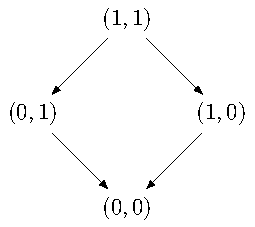
\includegraphics[scale = 0.8]{fig0}
                \caption{Одностоковая ориентация двумерного куба $G(\EE_2^2)$}\label{fig:hxy}
            }
        \end{figure}
        Если $h(0, 1) = (0, 1)$ или $h(0, 1) = (1,1)$, то в соответствии с предыдущими рассуждениями мы можем аналогичным образом рассмотреть проекцию $x_i \gets 0$, получим функцию $f(x) = h(0, x)[2]$, для которой $f(0) = 0$, $f(1) = 1$, следовательно $f(x) = x$, и мы нашли самодвойственную проекцию.







        Рассмотрим <<соседние>> по отношению к набору $\gamma = (0, \ldots, 0)$ наборы вида $e_i = (\underbrace{0, \ldots, 0}_{i-1}, 1, \underbrace{0, \ldots, 0}_{n-i})$.
        Если существует такой набор $e_i$, что $g_i(e_i) \ne g_i(0, \ldots, 0)$, то достаточно рассмотреть проекцию $\gf$ вида 
        \[
            h(x) = \proj_{1, \ldots, i-1, i+1, \ldots, n}^{0, \ldots, 0}(\gf) \colon \EE_2^1 \to \EE_2^1.
        \]
        Тогда $h(1) \ne h(0)$, а значит, $h(1) = \overline{h(0)}$.
        Таким образом, $h$~--- искомая самодвойственная проекция.

        Осталось рассмотреть случай, в котором для всех наборов $\widetilde{\gamma^i}$ выполнено условие $g_i(\widetilde{\gamma^i}) = g_i(\gamma)$.
        При этом если есть хотя бы один набор $\widetilde{\gamma^i}$, что $\gf(\widetilde{\gamma^i}) = \gf(\gamma)$, то мы можем перейти к размерности $n-1$, рассмотрев проекцию $\proj_{i}^{\overline{\gamma_i}}(\gf)$, для которой также выполняется условие утверждения.

        Следовательно, остается случай, при котором для каждого $\widetilde{\gamma^i}$ найдется хотя бы одна позиция $j$, для которой $g_j(\widetilde{\gamma^i}) \ne g_j(\gamma)$.
        Но в таком случае из неравенства следует, что $g_j(\widetilde{\gamma^i}) = \overline{g_j(\gamma)}$.
        Тогда возьмем любое $i$ и рассмотрим проекцию на те координаты $j$, для которых $g_j(\widetilde{\gamma^i}) = g_j(\overline{\gamma})$. 
        Индексов $j$ с таким условием будет не менее одного и не более $n-1$ по рассуждениям, приведенным ранее.
        Полученная проекция также будет удовлетворять условиям леммы и иметь меньший размер.
    \end{proof}

    \begin{theorem}
    \label{thm:self_proper}
        Семейство $\ff_n$ булевых функций правильно тогда и только тогда, когда каждая из его проекций $\proj^{a_1, \ldots, a_k}_{i_1, \ldots, i_k}(\ff)$ не является самодвойственной булевой функцией.
    \end{theorem}

    \begin{proof}
        Пусть $\ff_n$~--- правильное, $\gf = \proj^{a_1, \ldots, a_k}_{i_1, \ldots, i_k}(\ff)$~--- его проекция.
        Предположим, что $\gf$~--- самодвойственное.
        В таком случае, для любого $\alpha$ имеем $\gf(\alpha) = \overline{\gf(\overline{\alpha})}$.
        Тогда для $\gf$ нарушается свойство правильности, следовательно, $\ff$ не является правильным (поскольку любая проекция правильного семейства должна быть правильной, см. теорему~\ref{thm:proj}).

        Докажем утверждение в обратную сторону. 
        Для этого предположим, что $\ff_n$ не является правильным, и покажем, что в таком случае существует самодвойственная проекция.
        Так как $\ff_n$ не является правильным, то найдутся два набора $\alpha = (\alpha_1, \ldots, \alpha_n)$ и $\beta = (\beta_1, \ldots, \beta_n)$, такие что для всех индексов $i$, в которых $\alpha$ и $\beta$ различны, $\alpha_i \ne \beta_i$, выполнено условие $\ff_i(\alpha) \ne \ff_i(\beta)$.
        Рассмотрим проекцию $\gf$ семейства $\ff$ по тем координатам $j$, для которых $\alpha_j = \beta_j$. 
        Для семейства $\gf$ выполнено следующее условие: существует набор $\gamma$ такой, что $\gf(\gamma) = \overline{\gf(\overline{\gamma})}$.
        Тогда $\gf$ удовлетворяет условиям леммы~\ref{lemma:dual}, а значит, у этого семейства существует самодвойственная проекция, что и требовалось доказать.
    \end{proof}



\section{Другие критерии правильности}

    В настоящем разделе мы рассмотрим еще два критерия правильности:
    \begin{itemize}
        \item критерий в терминах неортогональности пространств (раздел~\ref{sec:nonortho}),
        \item критерий в терминах клик графов специального вида (раздел~\ref{sec:clique}).
    \end{itemize}


\subsection{О (не)ортогональности аффинных подпространств}
\label{sec:nonortho}

    Рассмотрим одно обобщение результата из работы~\cite{ruet2015asynchronous}, касающегося ортогональности подпространств булева куба (см. теорему~6 указанной работы).
    Указанный результат также был сформулирован для $\hupf$-сетей.
    На язык правильных семейств он <<переводится>> в более общей формулировке, но за счет некоторого ослабления понятия правильности в случае $k$-значных логик при $k \ge 3$ (см. определение~\ref{def:genericproper}).

    \begin{definition}
        \textbf{Аффинное подпространство.}
        Пусть $\xx, \yy \in Q^n$~--- два набора из $n$ элементов, обозначим через $[\xx, \yy]$ множество таких элементов $\vv \in Q^n$, что $\vv$ совпадает с $\xx$ в тех номерах координат, где $x_i = y_i$:
        \[
            [\xx, \yy] = \{\vv \in Q^n \mid v_i = x_i = y_i \text{ для всех $i$, где } x_i = y_i\}.
        \]
        Будем называть $[\xx, \yy]$ подпространством в $Q^n$.
    \end{definition}

    \begin{remark}
        В случае $Q = \ZZ_k$ нетрудно видеть, что $[\xx, \yy]$~--- это аффинное подпространство в $\ZZ_k^n$.
    \end{remark}
    
    \begin{definition}
        \textbf{Ортогональные пространства.}
        Пусть $[\xx, \yy]$ и $[\ww, \vv]$~--- два подпространства.
        Обозначим через $I = \{ i_1, \ldots, i_s \}$ все позиции, для которых $x_{i_j} \ne y_{i_j}$; обозначим через $L = \{ \ell_1, \ldots, \ell_t \}$ все позиции, для которых $w_{\ell_j} \ne v_{\ell_j}$.
        Будем говорить, что $[\xx, \yy]$ и $[\ww, \vv]$ ортогональны (и писать $[\xx, \yy] \perp [\ww, \vv]$), если выполнено следующее условие: $I \cap J = \varnothing$.
    \end{definition}

    \begin{example}[Ортогональность в случае $Q = \ZZ_k$]
        Рассмотрим случай $Q = \ZZ_k$.
        Тогда $[\xx, \yy]$ и $[\ww, \vv]$ являются аффинными подпространствами $\ZZ_k^n$.
        Пусть $[\xx, \yy] = \alpha + \mathcal{L}_1$, $[\ww, \vv] = \beta + \mathcal{L}_2$, тогда $[\xx, \yy] \perp [\ww, \vv]$ тогда и только тогда, когда $\mathcal{L}_1$ и $\mathcal{L}_2$ перпендикулярны (как векторные подпространства) относительно билинейной формы $\langle \xx \mid \yy \rangle = \sum_{i=1}^n x_i \cdot y_i$, то есть для любых $\xx \in \mathcal{L}_1$ и $\yy \in \mathcal{L}_2$ выполняется $\langle \xx \mid \yy \rangle = 0$.
    \end{example}

    После введения всех необходимых понятий мы можем привести необходимое условие правильности семейства в терминах ортогональных подпространств.

    \begin{theorem}
        \label{propos:nonortho}
        Если семейство $\ff_n \colon Q^n \to Q^n$ правильно, то для любых неравных $\xx, \yy \in Q^n$ выполнено условие не-ортогональности:
        \[
            [\xx, \yy] \not \perp [\xx \circ \ff_n(\xx), \yy \circ \ff_n(\yy)].
        \]
    \end{theorem}

    \begin{proof}
        Пусть $\ff$~--- правильное.
        Тогда по определению найдется такой индекс $i$, что $x_i \ne y_i$, но $f_i(x) = f_i(y)$.
        Но отсюда следует, что $x_i \circ f_i(x) \ne y_i \circ f_i(y)$.
        Следовательно, нашлась общая для $[\xx, \yy]$ и $[\xx \circ \ff(\xx), \yy \circ \ff(\yy)]$ координата $i$ такая, что $x_i \ne y_i$ и $x_i \circ f_i(x) \ne y_i \circ f_i(y)$.
        Это по определению влечет не-ортогональность соответствующих пространств.
    \end{proof}

    Обратное утверждение не всегда верно.
    \begin{example}
        Рассмотрим случай $k = 3$, $n=1$, $\ff(x) = x$, $\circ = +$.
        В таком случае:
        \begin{itemize}
            \item семейство $\ff$ не является правильным, поскольку зависит существенно от $x$,
            \item для семейства $\ff$ выполнено условие не-ортогональности: для любых неравных $x \ne y$ имеем
            \begin{gather*}
                [x, y] = \EE_3, \; x + f(x) = 2x \ne y + f(y) = 2y, \\
                [x + f(x), y + f(y)] = \EE_3.
            \end{gather*}
        \end{itemize}
    \end{example}

    Однако мы можем ввести понятие <<обобщенного правильного семейства>>, для которого условие <<обобщенной правильности>> будет эквивалентно условию отсутствия ортогональных аффинных подпространств указанного выше вида.

    \begin{definition}
    \label{def:genericproper}
        Пусть $Q$~--- квазигруппа.
        Будем называть семейство $\ff_n \colon Q^n \to Q^n$ обобщенно правильным, если для любых двух неравных наборов $\xx, \yy \in Q^n$ найдется индекс $i$, такой что выполнены условия:
        \[
            x_i \ne y_i, \quad x_i \circ f_i(\xx) \ne y_i \circ f_i(\yy).
        \]
    \end{definition}

    \begin{remark}
        Отметим два факта:
        \begin{itemize}
            \item правильные семейства являются обобщенно правильными: для правильных семейств найдется индекс $i$, что $x_i \ne y_i$, но $f_i(\xx) = f_i(\yy)$, откуда следует $x_i \circ f_i(x) \ne y_i \circ f_i(y)$;
            \item для булева случая понятия правильности и обобщенной правильности эквивалентны.
        \end{itemize}
    \end{remark}

    \begin{theorem}
        Семейство $\ff_n \colon Q^n \to Q^n$ является обобщенно правильным тогда и только тогда, когда выполнено условие не-ортогональности аффинных подпространств: для любых двух неравных наборов $\xx, \yy \in Q^n$ выполняется
        \[
            [\xx, \yy] \not \perp [\xx \circ \ff(\xx), \yy \circ \ff(\yy)]
        \]
    \end{theorem}

    \begin{proof}
        В прямую сторону утверждение доказывается аналогично утверждению~\ref{propos:nonortho}.
        В обратную сторону утверждение также является простым следствием определения ортогональности.
    \end{proof}

    \begin{theorem}
        \label{propos:bijection}
        Пусть семейство $\ff \colon Q^n \to Q^n$ обобщенно правильное.
        Тогда отображение $\sigma_{\ff} \colon Q^n \to Q^n$, переводящее $\xx \in Q^n$ в $\xx \circ \ff(\xx)$, является биективным.
    \end{theorem}

    \begin{proof}
        Докажем инъективность отображения $\sigma_{\ff}$: по определению обобщенной правильности для люыбх $\xx \ne \yy$ найдется индекс $i$ такой, что 
        \[
            x_i \circ f_i(\xx) = \sigma_{\ff}(\xx)[i] \ne \sigma_{\ff}(\yy)[i] = y_i \circ f_i(\yy).
        \]
        Биективность следует из конечности $Q^n$.
    \end{proof}


\subsection{Кликовое представление правильных семейств}
\label{sec:clique}

    В работах~\cite{sikiric2007cube, mathew2013enumerating} изучались \textquote{кубические замощения} пространства (cube tilings), а также подсчитывалось количество подобных неэквивалентных замощений (число классов изоморфизма) для разных размерностей замощаемого пространства (см. таблицу~\ref{tab:counttilings})
    \begin{table}[h]
        \centering
        \captionsetup{justification=centering} % выравнивание подписи по-центру
        \caption{\label{tab:counttilings} Число неэквивалентных замощений пространства размерности $n$.}
        \begin{tabular}{|c|c|}
            \toprule
            Размер $n$  & Число замощений \\
            \midrule
            $n = 1$ & 2 \\
            \midrule
            $n = 2$ & 12 \\
            \midrule
            $n = 3$ & 744 \\
            \midrule
            $n = 4$ & 5541744 \\
            \midrule
            $n = 5$ & 638560878292512 \\
            \bottomrule
        \end{tabular}
    \end{table}
    
    Для $n = 1,2,3,4$ количество замощений пространства размерности $n$ совпадает с числом правильных булевых семейств размера $n$.
    Это совпадение неслучайно: в работе~\cite{borzechowski2022universal} было показано, что одностоковые ориентации булевых кубов находятся в биективном соответствии с замощениями пространства гиперкубами, а именно, было показано, что каждой одностоковой ориентации можно однозначно сопоставить клику в некотором графе специального вида (т.н. графы Келлера, см.~\cite{corradi1990combinatorial}).
    Обобщим этот результат на случай $k$-значный случай: покажем, что правильные семейства функций $k$-значной логики находятся в биективном соответствии с кликами графов, построенных аналогично графам Келлера (и совпадающих с этими графами при $k = 2$).

    \begin{definition}
        Пусть $G = (V, E)$~--- некоторый граф.
        Клика на $m$ вершинах в графе $G$~--- это подмножество вершин $V' \subseteq V$ размера $m$, такое что каждые две вершины $v, w \in V'$ соединены ребром в $G$: $\{v, w\} \in E$.
    \end{definition}

    Рассмотрим следующее обобщение графов Келлера на $k$-значный случай.

    \begin{definition}
        Зададим обобщенный граф Келлера $G(k, n)$ следующим образом:
        \begin{itemize}
            \item множество вершин графа $V$~--- наборы чисел от $0$ до $k^2-1$ длины $n$: 
            \[
                V = \EE_{k^2}^n;
            \]
            \item ребро $\{v, w\} \in E$, тогда и только тогда, когда найдется координата $i$, $1 \le i \le n$, что выполнены два условия: 
            \[
                v_i \equiv w_i \mod \; k, v_i \ne w_i.
            \]
        \end{itemize}
    \end{definition}

    Будем рассматривать правильные семейства $\ff_n$ размера $n$ на $\EE_k^n$.
    Покажем, что они находятся во взаимно-однозначном соответствии с \textbf{кликами} в графе $G(k,n)$ размера $k^n$ (по правильному семейству строится клика в графе $G(k, n)$, и наоборот, по каждой клике размера $k^n$ в $G(k, n)$ задается правильное семейство на $\EE_k^n$).

    \begin{theorem}
        Каждой клике на $k^n$ вершинах в графе $G(k, n)$ можно поставить в биективное соответствие некоторое правильное семейство $\ff_n$ размера $n$ на $\EE_k^n$.
    \end{theorem}

    \begin{proof}
        Доказательство будет состоять из двух частей.
        Сначала рассмотрим вложение множества правильных семейств в множество клик графа $G(k, n)$, а затем покажем обратное: по каждой клике графа $G(k, n)$ построим некоторое правильное семейство $\ff_n$ размера $n$ на $\EE_k^n$.

        Рассмотрим некоторое правильное семейство $\ff = (f_1, \ldots, f_n)$ на $\EE_k^n$.
        Каждому набору $\xx = (x_1, \ldots, x_n) \in \EE_k^n$ поставим в соответствие набор из $\EE_{k^2}^n$ следующим образом.
        Для $a, b \in \EE_k$ определим число $\phi(a, b) =  k \cdot a + b \in \EE_{k^2}$, тогда набору $\xx$ поставим в соответствие набор 
        \[
            \xx \to \Phi_{\ff}(\xx) = \left( \phi(x_1, f_1(\xx)), \ldots, \phi(x_n, f_n(\xx)) \right) \in \EE_{k^2}^n.
        \]
        Повторим указанный процесс для каждого $\xx \in \EE_k^n$ и получим набор вершин в графе $G(k, n)$, построенный по семейству $\ff$.

        Полученное отображение $\Phi_{\ff}$ в множество вершин $V$ инъективно для каждого фиксированного правильного семейства $\ff$: если $\xx \ne \yy$, то $\Phi_{\ff}(\xx) \ne \Phi_{\ff}(\yy)$.
        Это следует из свойства правильности: найдется индекс $1 \le i \le n$, что $x_i \ne y_i$, но $f_i(\xx) = f_i(\yy)$, а значит, $\phi(x_i, f_i(\xx)) = k \cdot x_i + f_i(\xx) \ne k \cdot y_i + f_i(\yy) = \phi(y_i, f_i(\yy))$.
        Заметим также, что для полученных элементов выполняется условие 
        \[
            \phi(x_i, f_i(\xx)) \ne \phi(y_i, f_i(\yy)), \quad \phi(x_i, f_i(\xx)) \equiv \phi(y_i, f_i(\yy)) \; \mod k,
        \]
        а значит, полученные вершины графа соединены ребром в $G(k, n)$.
        Таким образом, отображение $\Phi_{\ff}$ задает по правильному семейству $\ff$ некоторый подграф графа $G(k ,n)$ на $k^n$ вершинах, причем любые две вершины в подграфе соединены ребром, а значит, составляют клику.

        Отображение $\ff \to \Phi_{\ff}$ также является инъективным (определяет различные клики при разных правильных семействах): если $\ff \ne \gf$, то существует $\xx \in \EE_k^n$, такой что $\ff(\xx) \ne \gf(\xx)$, но тогда $\Phi_{\ff}(\xx) \ne \Phi_{\gf}(\xx)$, и ни для какой точки $\yy \in \EE_k^n$ не может выполняться равенство $\Phi_{\ff}(\xx) = \Phi_{\gf}(\yy)$, а значит, точки $\Phi_{\ff}(\xx)$ нет в клике, задаваемой отображением $\Phi_{\gf}$.

        Рассмотрим теперь обратное отображение: каждому элементу $a \in \EE_{k^2}$ поставим в соответствие пару $(x, y) \in \EE_k^2$ вида 
        \[
            a \to \psi(a) = (a \text{ div } k, \; a \mod \; k),
        \]
        а каждому элементу $\vv = (v_1, \ldots, v_n) \in \EE_{k^2}^n$~--- пару векторов 
        \begin{gather*}
            (\xx, \yy) = \Psi(\vv) \in \left( \EE_{k}^n \right)^2, \\
            (x_i, y_i) = \psi(v_i), \; 1 \le i \le n.
        \end{gather*}
        Покажем, что при этом отображении клики перейдут в правильные семейства.

        Во-первых, такое отображение на кликах инъективно: если $\vv \ne \ww$, $\Psi(\vv) = (\xx, \alpha)$, $\Psi(\ww) = (\yy, \beta)$, $\vv$ и $\ww$ соединены ребром в графе $G(k, n)$, то найдется индекс $i$, для которого $v_i \ne w_i$, но $v_i \equiv w_i \mod k$, а значит, $x_i \ne y_i$.
        В силу того, что в каждой рассматриваемой клике $k^n$ вершин, указанное отображение ставит ей в соответствие множество пар $\{ (\xx, \alpha) \in \left( \EE_{k}^n \right)^2 \mid \xx \in \EE_k^n \}$, где первые элементы пар $\xx$ пробегают все множество $\EE_k^n$.

        Во-вторых, если мы интерпретируем второй элемент пары $\alpha$ как значение некоторого отображения $\ff \in P_k^n$ на элементе первой пары $\xx$ (т.е. $(\xx, \alpha) = (\xx, \ff(\xx))$), то семейство $\ff$ будет правильным, покажем это.
        Рассмотрим два неравных набора $\xx \ne \yy \in \EE_k^n$, а также их прообразы при отображении $\Psi$: $ \vv = \Psi^{-1}(\xx, \alpha)$, $ \ww = \Psi^{-1}(\yy, \beta)$.
        Для векторов $\vv$ и $\ww$ найдется индекс $1 \le i \le n$, для которого $v_i \ne w_i$, но $v_i \equiv w_i \mod k$ (поскольку $\vv$ и $\ww$ соединены ребром в $G(k, n)$), а значит, $x_i \ne y_i$, но при этом $\alpha_i = \beta_i$, т.е. выполнено условие правильности.
    \end{proof}

    \TODO{подумать, как связаны изоморфизмы графа $G(k, n)$ и изометрии правильных семейств.}

    \TODO{что хорошего ещё можно сказать про это всё?}

\section*{Выводы}

    В этой главе мы рассмотрели несколько альтернативных способов описания булева правильного семейства:
    \begin{itemize}
        \item характеризация в терминах одностоковой ориентации (т.н.~$\mathsf{USO}$-ориентации булева куба),
        \item характеризация в терминах булевой сети с наследственно неподвижной точкой (т.н.~$\hupf$-сети),
        \item характеризация в терминах булева отображения, каждая проекция которого не является самодвойственной,
        \item характеризация в терминах клик обобщенных графов Келлера.
    \end{itemize}
    Также было введено понятие обобщенно правильного семейства и его альтернативная характеризация в терминах ортогональности подпространств (в случае $k=2$ понятие обобщенно правильного семейства совпадает с понятием правильного семейства).

    Таким образом, один и тот же объект (правильные семейства) может быть рассмотрен сразу с нескольких точек зрения, а результаты, полученные в рамках одного \textquote{языка}, могут быть перенесены на другой \textquote{язык} (часто даже в более общем виде).
    При этом геометрическая интуиция позволяет ввести некоторые новые классы семейств, такие как рекурсивно и локально треугольные семейства, а также доказать некоторые свойства правильных семейств (например, $\mathsf{coNP}$-полноту задачи распознавания правильности по схеме из функциональных элементов или оценку на число булевых правильных семейств).
